\documentclass[10pt,conference,compsocconf]{IEEEtran}

\usepackage{hyperref}
\usepackage{graphicx}	% For figure environment
\usepackage{amsmath}
\usepackage{amssymb}
\usepackage{float}
\usepackage{url}
\newcommand{\beginsupplement}{%
	\setcounter{table}{0}
	\renewcommand{\thetable}{S\arabic{table}}%
	\setcounter{figure}{0}
	\renewcommand{\thefigure}{S\arabic{figure}}%
}

\begin{document}
\title{Extreme Wind Analysis}

\author{
	Matthias Minder, Yves Rychener
}

\maketitle


\begin{abstract}

\end{abstract}

\section*{Introduction} 
Modeling extreme weather events is of interest for a variety of applications, such as risk assessment for insurance companies or conception of preventive measures. In particular, questions about how often a particular event will occur, how severe events can get, and whether there are seasonal or year-dependent trends are of interest. Within the scope of this report, we will address these questions for extreme thunderstorms on a 1° longitude and 1° latitude grid cell with south-west coordinates 38° latitude and -100° longitude, situated in central Kansas. The measured quantities are the Connective Available Potential Energy ($CAPE$) and the Storm Relative Helicity ($SRH$), which have to be simultaneously high for severe thunderstorms to occur. Three-hourly time series of these events are taken into account from January 1st 1979 at 00:00 to December 31st 2015, 21:00. 
\par
In particular, we will study the structure variable denoted $PROD$ given by $PROD = \sqrt{CAPE} \times SRH$. It captures concurrently high values of $SRH$ and $CAPE$, and is thus apt for modeling the risk of thunderstorms. Every month will be treated separately in order to capture seasonal differences. To model extreme values, a generalized extreme value distribution will be fitted to the monthly maxima of $PROD$ using maximum likelihood estimation as well as Bayesian approaches. Moreover, the generalized extreme value distribution will be fitted to the $r$-largest order statistic for every month to determine whether that improves the fit. Subsequently, we will assess dependence of $PROD$ upon time and the NINO 3.4 index, an established indicator of the El-Niño Southern Oscillation ($ENSO$). 
\par
Following this, $CAPE$ and $SRH$ are considered separately. We will study whether they are asymptotically dependent, before fitting bivariate models to the joint extremes of $CAPE$ and $SRH$. 
Finally, 50- and 100-year return levels of $PROD$ are calculated based on fitting a point process model to $PROD$ with maximum likelihood estimation, based on the Bayesian fit, and based on simulated values of $CAPE$ and $SRH$ from the bivariate model fitted before. 

\section*{Preliminary Analysis}
\begin{figure}
	\centering
	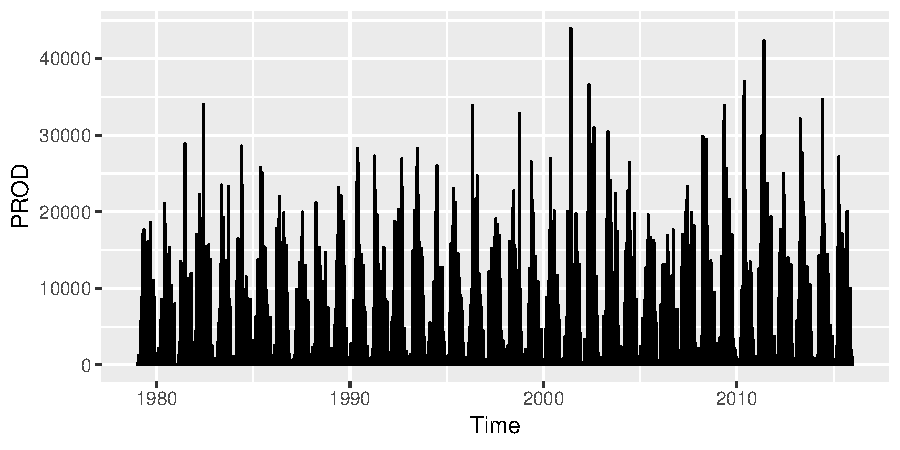
\includegraphics[width=0.35\textwidth]{../plots/full_time_series.pdf}
	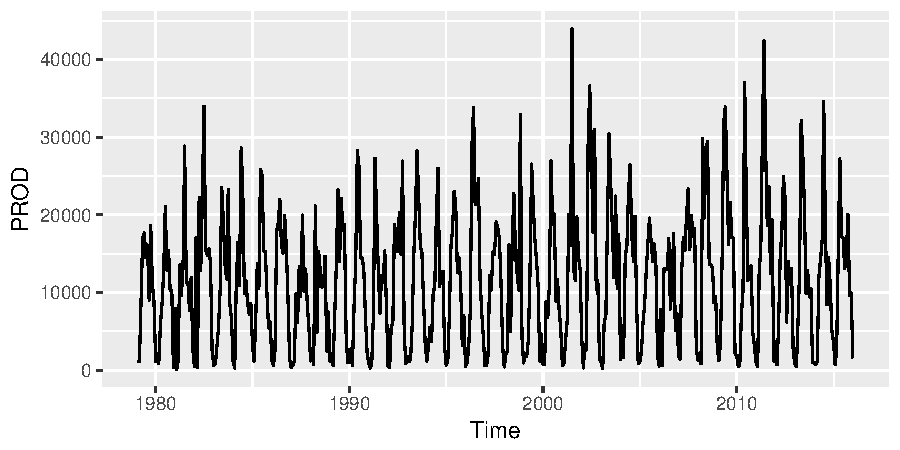
\includegraphics[width=0.35\textwidth]{../plots/monthly_max_series.pdf}
	\caption{Three-hourly values (top) and monthly maxima (bottom) of $PROD$ values for the entire analyzed period.}
	\label{fig:timeseries}
\end{figure}
Plotting the full time series and the monthly maxima as shown in Figure \ref{fig:timeseries} clearly shows the seasonality of the data, with high values of $PROD$ occurring mainly during summer. This clearly shows the necessity of separate treatment of months. Moreover, there seems to be some upward trend following time, with more extreme values of $PROD$ in recent years.

\section*{Fitting Generalized Extreme Value Distribution to PROD}
In order to understand the behavior of the monthly maxima, we fitted a generalized extreme value (GEV) distribution to $PROD$ for each month separately with three different approaches. 
\begin{figure}
	\centering
	\textbf{January}\\
	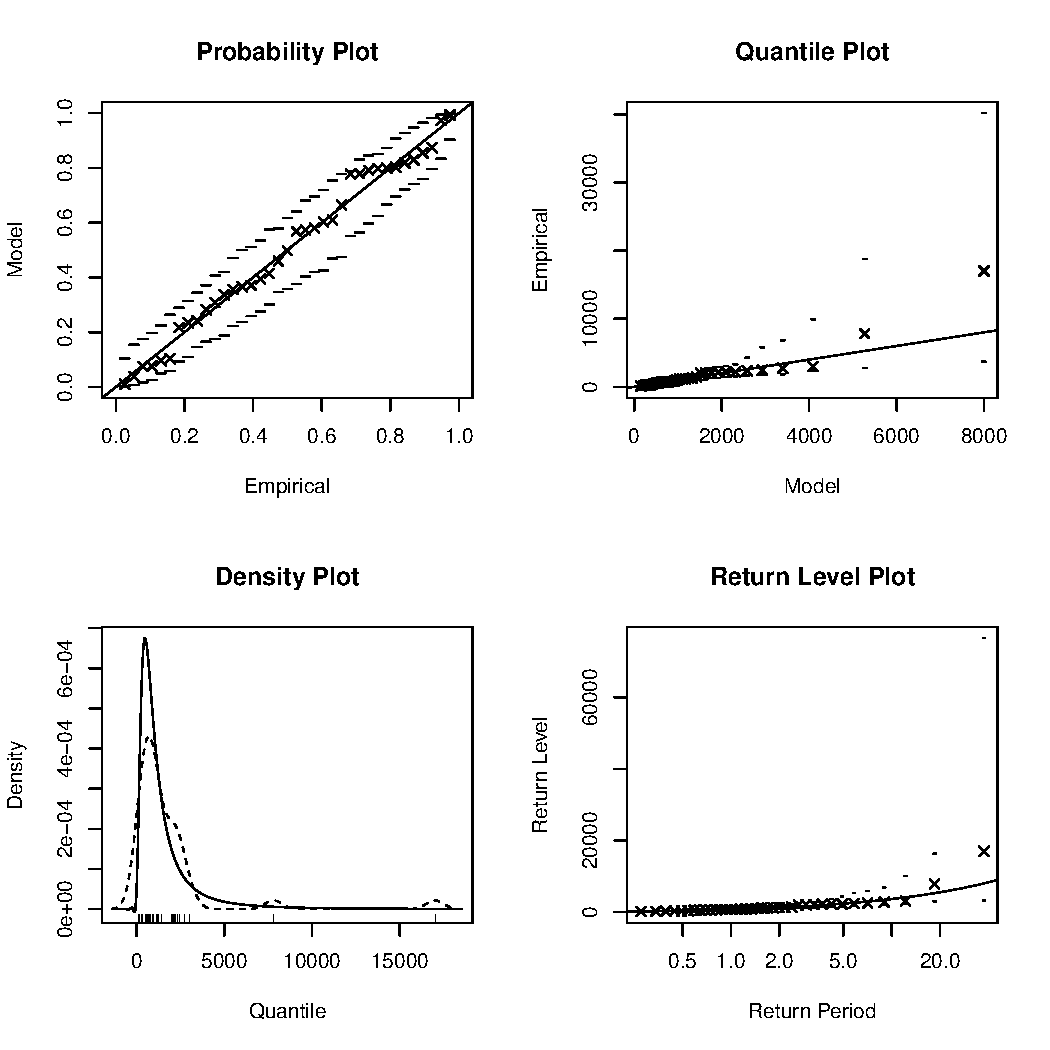
\includegraphics[width=0.35\textwidth]{../plots/monthly_mle_diag/01_monthly_mle_diag.pdf}\\
	\textbf{December}\\
	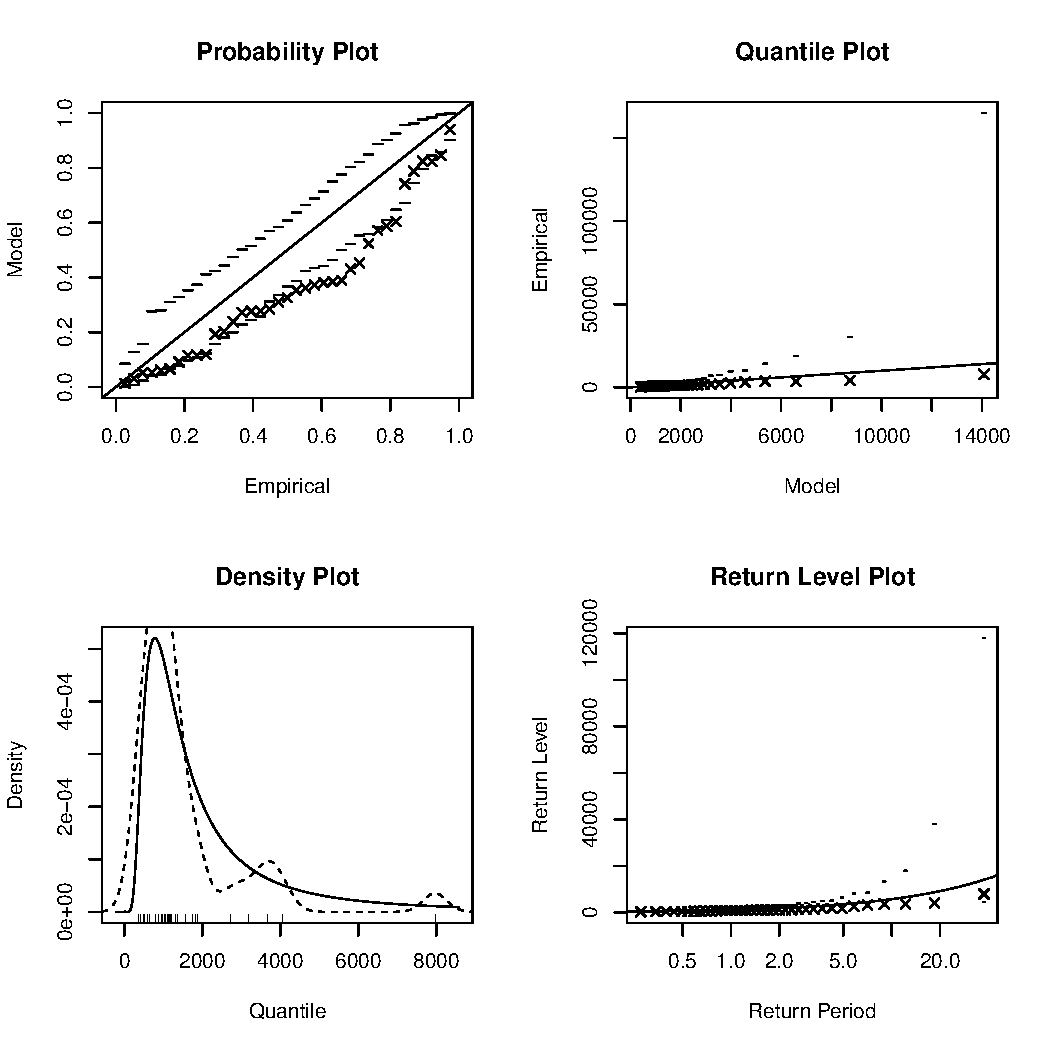
\includegraphics[width=0.35\textwidth]{../plots/monthly_mle_diag/12_monthly_mle_diag.pdf}
	\caption{Diagnostic plots for fitting GEV to the data using maximum likelihood estimation for January (top) and December (bottom). Whereas in January the model fits the data, as shown by the fact that the observed values are within the confidence range for probability plot, this is not the case for December, indicating a poor fit.}
	\label{fig:mle_diag}
\end{figure}
\par
First, we fitted the values using maximum likelihood estimation. Fitting was done using the evd package in R, using the Nelder-Mead optimization method and standard parameters \cite{evd}. The quality of the fit was assessed using diagnostic plots, as shown for January and December in Figure \ref{fig:mle_diag}. The model performed well with the exception of September and December: In September optimization didn't succeed, whereas in December the observed values lie outside of the given confidence intervals, as shown in Figure \ref{fig:mle_diag}. For both of these months, no standard error could be calculated due to singularity of the observed Fisher information matrix. Since we expect some continuity over the course of the year, the problem wasn't further investigated as inferences for the missing months can be made from their adjacent months. 
\par
Then, we fitted the values using the Metropolis-Hastings algorithm. As a prior for the three parameters, a normal distribution with mean zero and a diagonal covariance matrix was used.
Here, we will give an intuitive explanation of the Metropolis-Hastings algorithm; for a more detailed and mathematically rigorous explanation, please refer to slides 82-86 of the course slides.
This algorithm creates a Markov chain with stationary distribution $\pi(x)$, where $\pi(x)$ is also the desired distribution of the parameters of our model. The transition probability from $x$ to $y$ is $p(x,y)=\alpha(x,y) q(x,y)$, where $\alpha(x,y)$ is the acceptance rate, and $q(x,y)$ is the proposition density. We can select the proposition density $q(x,y)$ ourselves, usually a normal distribution is chosen, the acceptance rate can be shown to be $\alpha(x,y)=min(\frac{\pi(y) q(y,x)}{\pi(x) q(x,y)},1)$.
\par
We can imagine the sampling as follows: An agent is navigating the Markov chain. At every iteration, it will sample a proposed step to take from the distribution $q(x,y)$. Then, with probability $\alpha(x,y)$, it is allowed to take said step and move to a new state. With probability $1-\alpha(x,y)$, the step is rejected and we stay at the current state. We can estimate the (unknown) stationary distribution of the chain by navigating $n$ iterations and keeping track of the empirical state distribution. As $n \to \infty$ (or in practice for big $n$), we converge to the true stationary distribution. The proposal standard deviation dictates how big the proposal steps are. If the agent wants to take steps that are too big, he gets rejected all the time and cannot explore the chain. If the proposal steps are too small, he cannot fully explore the chain since $n$ has to be finite in order to finish our calculation. In practice, we have to remove some "burn in", since we may start very far away from the stationary distribution. Also, thinning is applied, since each state is dependent on the preceding state, resulting in high autocorrelation. 
\par
The proposal standard deviations were fine-tuned to obtain acceptance rates between 0.2 and 0.4. In order to avoid having to fine-tune every month separately, we implemented the following very simple optimization algorithm: If the acceptance rates for a given parameter were too high, the proposal standard deviation for said parameter were multiplied with 1.5. In the opposite case for low acceptance rates, the proposal standard deviation was divided by 2. The Metropolis-Hastings algorithm was run with 30'000 iterations. The chain was thinned with a factor 300 in order to avoid dependence between steps of the Markov chain. The thinning was validated with autocorrelation plots (not shown). The final parameter was determined to be the median of the posterior distribution, in order to be robust to outliers and be more adapted to skewed distributions. 
\par

\section*{Dependence of PROD on Time and ENSO}
A dependence test of $PROD$ can be done by likelihood ratio test. For this, we test the model with constant parameters (null hypothesis) against the model with linear dependence for the location parameter (alternative hypothesis), i.e. $\eta = \eta_0 + \eta_1*x$, where $x$ is the trend. When taking a linear trend, we center and renormalise the trend  as recommended in the \textit{fgev} help files. We employ the Bonferroni multiple testing method to take into account the multiple tests at 95\% significance level (arising from the different months tested). Figure \ref{fig:dependance_test} displays the different ratios and the significance level (red) for the 95\% test. We see that the test is rejected in October for $ENSO$ dependence, and in December for time dependence. Independence can however not be ruled out for the other months. We also test a step function trend, simulating a regime change. The step function trend is calculated as $x_{step} = step(renormalised(x))$. Here the step function is defined as $step(x) = \begin{cases} 1 & if x>0\\ 0 & otherwise \end{cases}$. The formula for the corrected $\eta$ is now $\eta = \eta_0 + \eta_1*x_{step}$. With a step trend, the independence assumption can only be rejected for December time dependence (Figure \ref{fig:dependance_test_step}).
DA SÖTT NO E CONCLUSION HERE...

\begin{figure}
	\centering
	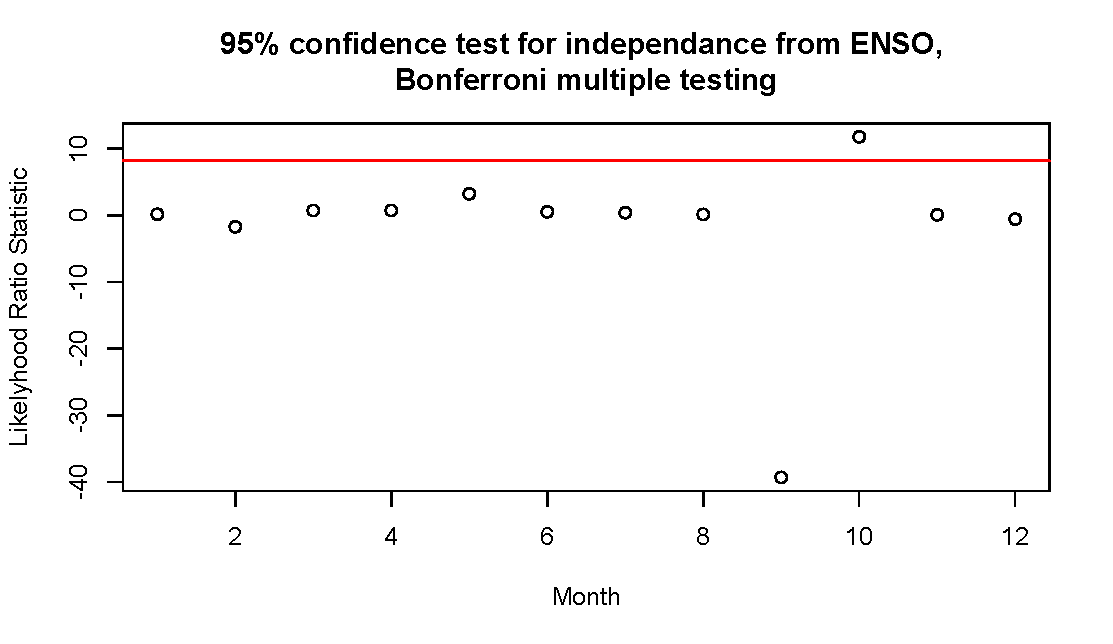
\includegraphics[width=0.35\textwidth]{../plots/enso_dependance.pdf}\\
	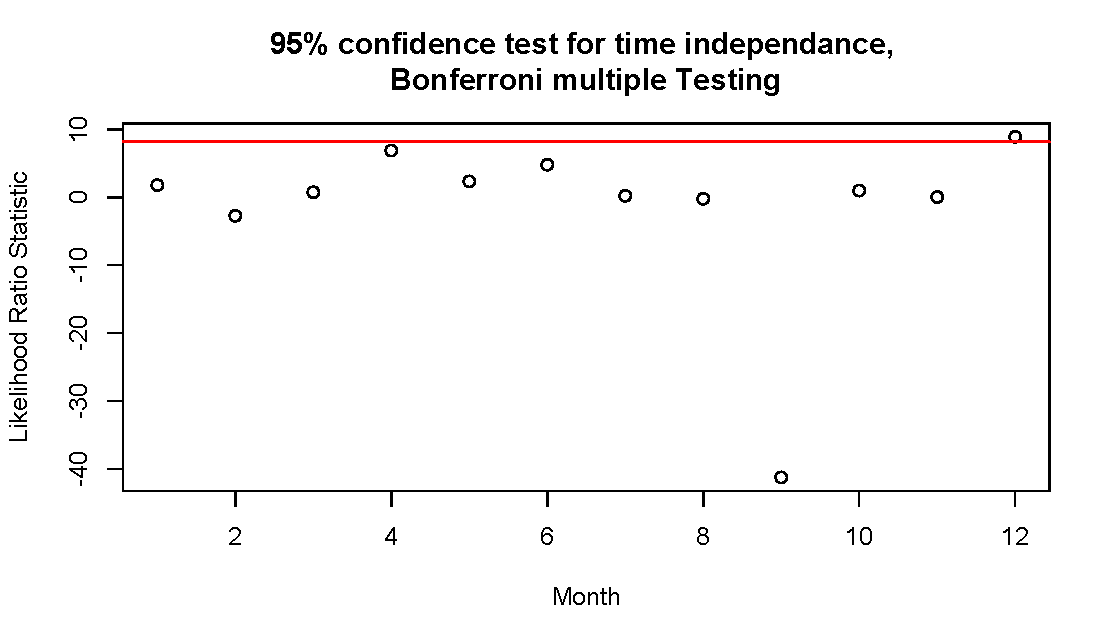
\includegraphics[width=0.35\textwidth]{../plots/time_dependance.pdf}
	\caption{Plots for likelihood ratios and 95\% significance levels for linear dependence}
	\label{fig:dependance_test}
\end{figure}

\begin{figure}
	\centering
	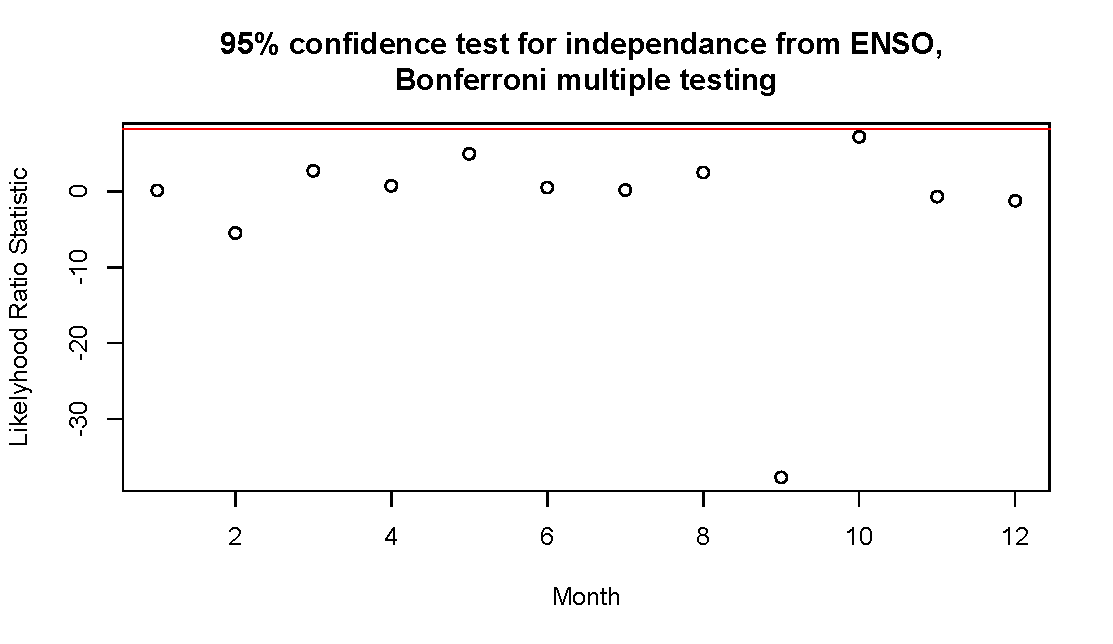
\includegraphics[width=0.35\textwidth]{../plots/enso_dependance_step.pdf}\\
	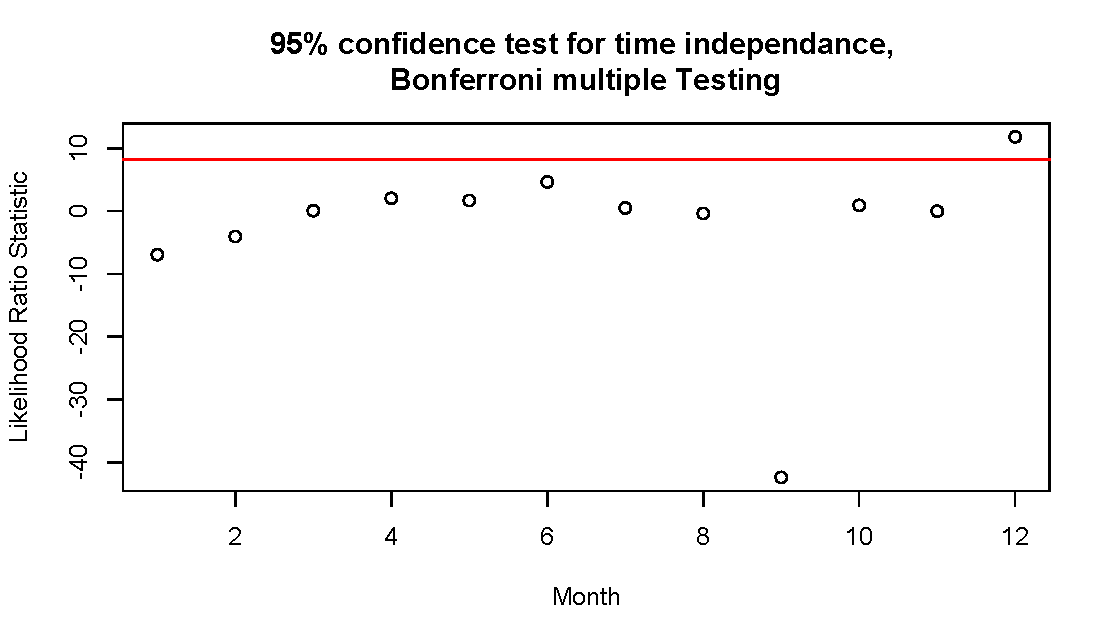
\includegraphics[width=0.35\textwidth]{../plots/time_dependance_step.pdf}
	\caption{Plots for likelihood ratios and 95\% significance levels for linear dependence}
	\label{fig:dependance_test_step}
\end{figure}

\section*{Dependence of CAPE and SRH}
Asymptotic dependence (or independence) of bivariate maxima of two random variables can be estimated using $\chi$ and $\bar{\chi}$ plots as provided by the \texttt{chiplot} function of the \texttt{evd} package \cite{evd}. The $\chi$ plot estimates for two random variables, $X \sim F_X$ and $Y \sim F_Y$, the probability 
\begin{align*}
	P\{F_X (X) > u | F_Y (Y) > u\}
\end{align*}
for a given probability threshold $u$. The asymptotic behavior is observed as the upper support point of the distributions are attained, as $u \to 1$. If the maxima are independent, the quantity $\lim_{u \to 1} \chi(u) = 0$. Whereas $\chi(u)$ can measure the strength of the dependence, the rate at which $\chi(u) \to 0$ as $u \to 1$ is measured by the $\bar{\chi}$ plot. Generally we can say that for asymptotic independence $\lim_{u \to 1} \bar{\chi}(u) \to 0$, and for asymptotic dependence $\lim_{u \to 1} \bar{\chi}(u) \to 1$. 
%The value of interest is $\chi = \lim_{u \to 1} \chi(u)$. For independence, $\chi \to 0$, since as $u \to 1$, $P\{F_X(x)>u | F_Y(y)>u\} \to \chi$. $\chi$ can distinguish the strength of dependence, but not the rate at which $\chi(u) \to 0$ as $u \to 1$. For this we can use the $\bar{\chi}$ plot. Generally we can say that for asymptotic independence $\lim_{u \to 1} \bar{\chi}(u) \to 0$, and for asymptotic dependence $\lim_{u \to 1} \bar{\chi}(u) \to 1$. (Source Slides 239-242 of the lecture notes)
\par
Our chi plots for all months look very similar. They suggest asymptotic independence between $CAPE$ and $SRH$ since $\lim_{u \to 1} \chi(u) \to 0$ and $\lim_{u \to 1} \bar{\chi}(u) \to 0$. Figure \ref{fig:cape_srh_chi} shows two representative examples of $\chi$ and $\bar{\chi}$ plots, for May and November. 

\begin{figure}
	\centering
	\textbf{May}\\
	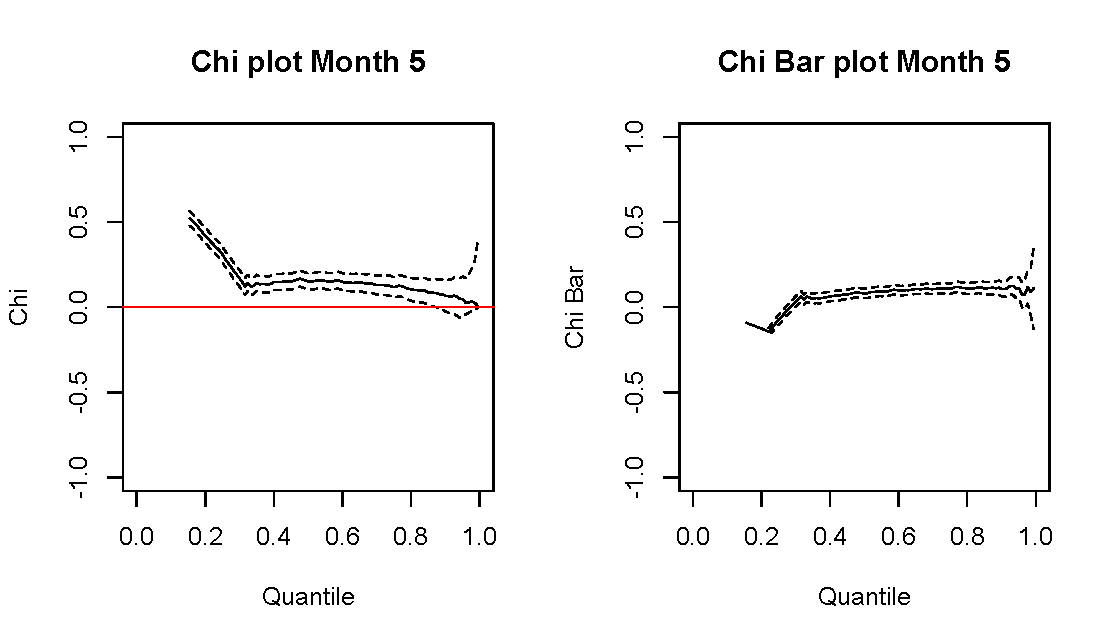
\includegraphics[width=0.35\textwidth]{../plots/May_chi.pdf}\\
	\textbf{November}\\
	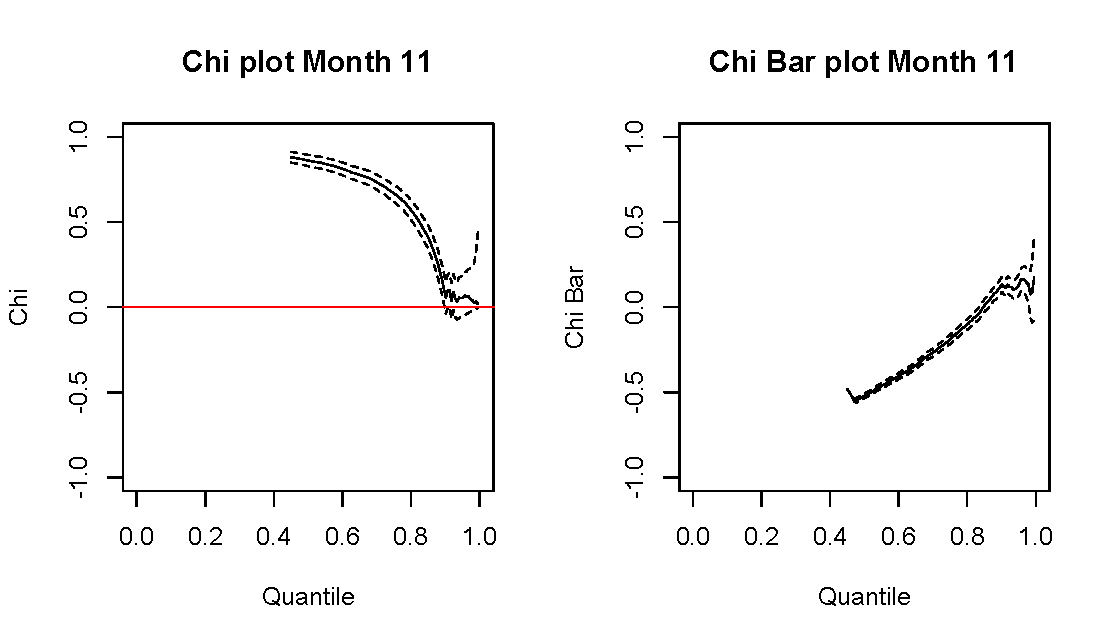
\includegraphics[width=0.35\textwidth]{../plots/November_chi.pdf}
	\caption{Representative examples for chi plots for $CAPE$ and $SRH$, both suggesting asymptotic independence since they approach 0 as the quantile $u \to 1$.}
	\label{fig:cape_srh_chi}
\end{figure}

\section*{Bivariate Fitting of CAPE and SRH}
Whereas until now only the single structure variable $PROD$ was considered, in this section its two components $CAPE$ and $SRH$ are taken separately. A bivarate extreme value distribution is  fitted to the data with the \texttt{fbvevd} function of the \texttt{evd} package \cite{evd}, using six different parametric link functions. The tested link functions were logistic (log), asymmetric logistic (alog), negative logistic (neglog), bilogistic (bilog), Coles-Tawn (ct) and negative bilogistic models (negbilog), and thus comprised symmetric and asymmetric models. The quality of the fit using different link functions were compared using the Akaike Information Criterion (AIC), as shown in Table \ref{table:cape_srh_AIC}.
\par
We observe that the negative logistic link function is the best or among the best fits for all months. This suggests that the introduction of asymmetry between $CAPE$ and $SRH$ doesn't improve the fit. In order to treat all months consistently, fits using this link function for all months were used for subsequent analysis. 
\begin{table}[]
\begin{tabular}{lllllll}
Month     & log       & alog      & neglog    & bilog     & ct        & negbilog  \\
January   & 920.4  & 921.3  & 920.1  & 920.3  & 921.0  & 920.3  \\
February  & 993.3  & 997.1  & 993.5  & 995.3  & 996.2  & 994.8  \\
March     & 1070.1 & 1074.2 & 1069.5 & 1072.2 & 1074.1 & 1071.6 \\
April     & 1064.8 & 1068.7 & 1064.6 & 1066.1 & 1066.2 & 1066.3 \\
May       & 1066.5 & 1070.4 & 1066.5 & 1068.3 & 1071.0 & 1068.2 \\
June      & 1043.3 & 1047.0 & 1043.4 & 1040.7 & 1043.1 & 1045.5 \\
July      & 1047.0 & 1044.9 & 1046.7 & 1046.2 & 1048.4 & 1046.5 \\
August    & 1029.2 & 1033.0 & 1029.4 & 1031.1 & 1031.3 & 1031.2 \\
September & 1056.0 & 1059.6 & 1055.7 & 1058.1 & 1059.9 & 1057.3 \\
October   & 1038.0 & 1042.0 & 1037.6 & 1037.6 & 1039.3 & 1038.5 \\
November  & 1012.4 & 1016.4 & 1012.7 & 1014.5 & 1015.1 & 1014.1 \\
December  & 892.7  & 896.7  & 892.5  & 894.9  & 895.5  & 894.3
\end{tabular}
\caption{AIC comparison of different link function models}
\label{table:cape_srh_AIC}
\end{table}
Note that for this fit, we extracted for each month the maximal $SRH$ value and the maximal $CAPE$ value and fitted the distribution to this data pair. However, the monthly maximum of these two independent variables don't necessarily correspond to the same event. We have therefore to be careful when drawing conclusions, since the "observations" we fit the models to often don't actually exist.
\par
Before, we estimated the dependence between CAPE and SRH. We can also these results with the fits we just made. For this we will use the dependence parameter $\alpha$ from the logistic model. For this model, we know that for independence $\alpha \to 1$ and for complete dependence $\alpha \to 0$. In Figure \ref{fig:cape_srh_dependance_logistic} we plot the dependence parameters with 95\% confidence bands. This suggests that independence between $SRH$ and $CAPE$ cannot be ruled out, in accordance to our analysis in the previous paragraph.

\begin{figure}
	\centering
	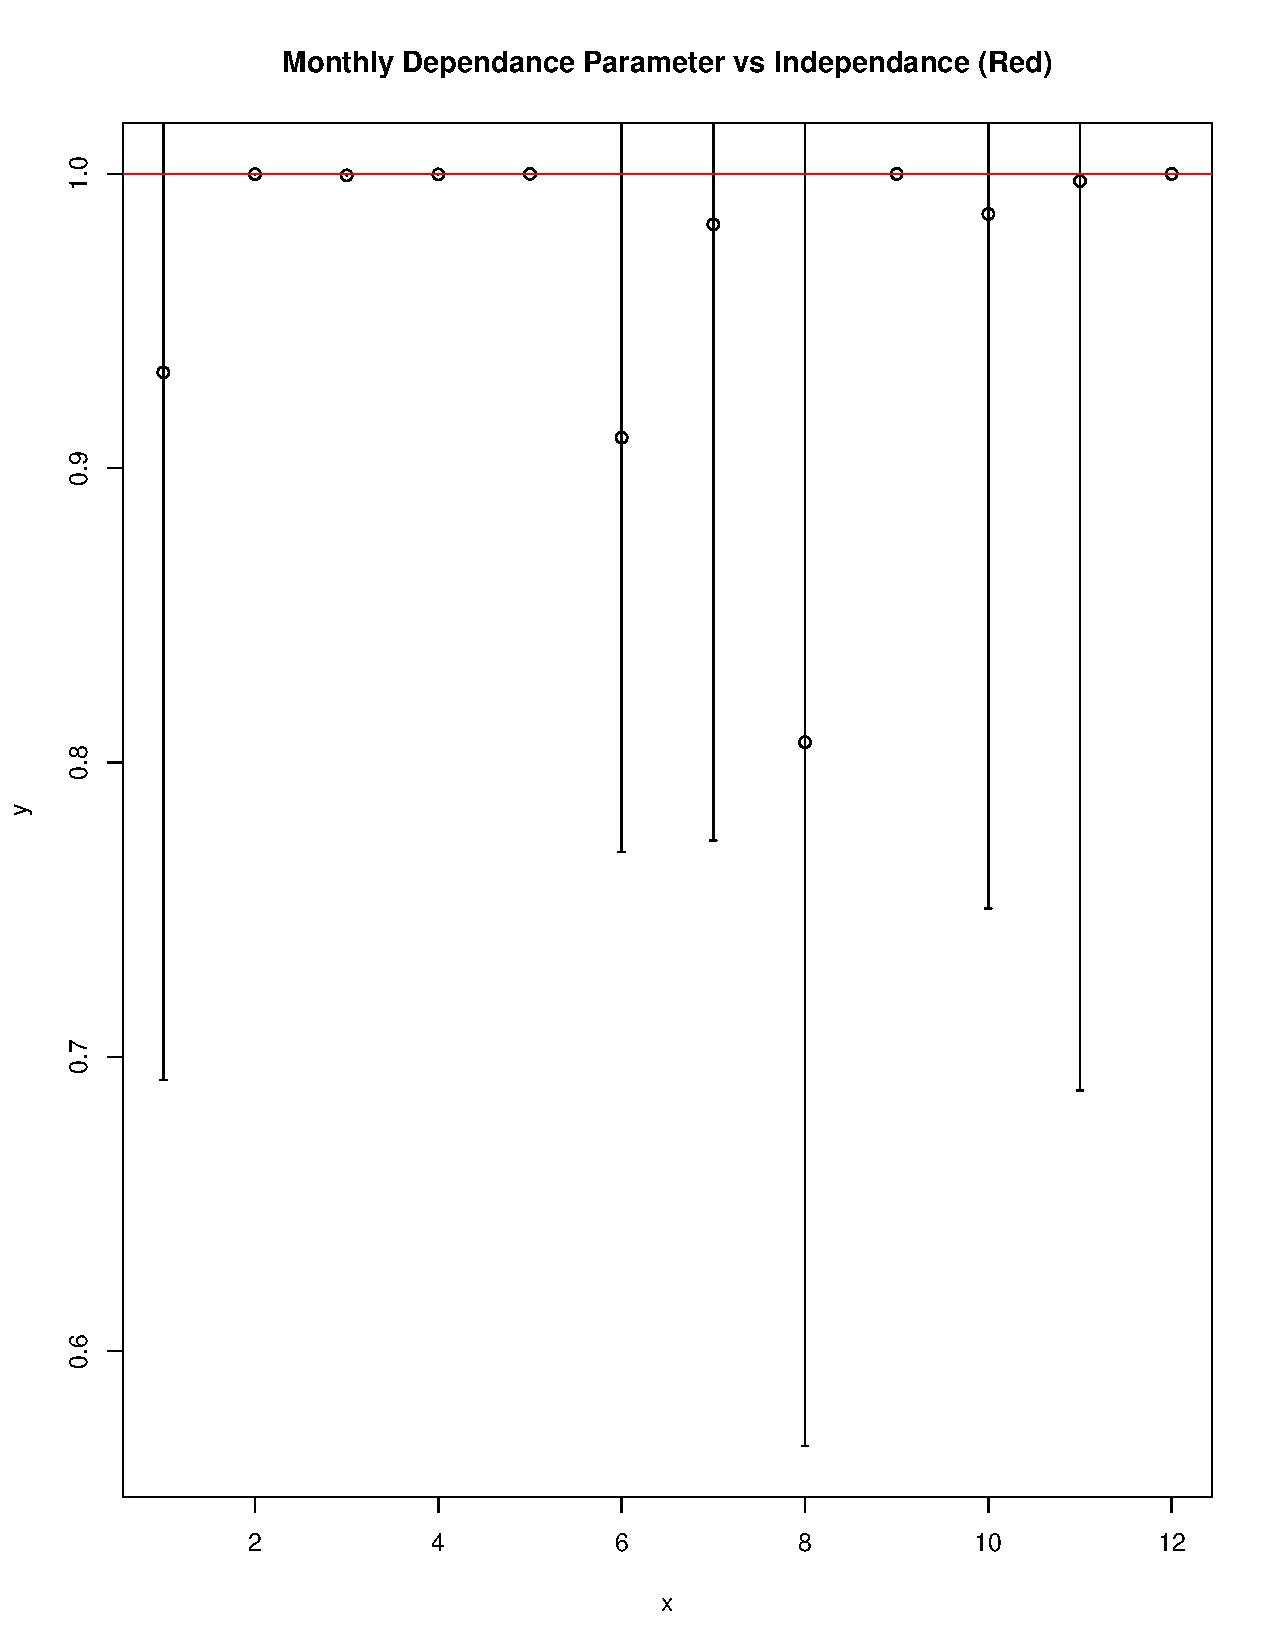
\includegraphics[width=0.35\textwidth]{../plots/dependance_parameter_cape_srh_logistic.pdf}
	\caption{Monthly dependence parameter $\alpha$ with 95\% confidence bands.}
	\label{fig:cape_srh_dependance_logistic}
\end{figure}

\section*{Calculation of Return Levels}
It is of interest to estimate the return levels of extreme events, 


\section*{Impact by Using Variable Transfromations}
We argue (without testing this explicitly), that using a $log(\cdot)$ transformation on $CAPE$, $SRH$ and $PROD$ would not change our analysis much. If $CAPE$ and $SRH$ arise from a joint distribution $F$, then $log(CAPE)$ and $log(SRH)$ arise from a distribution $F'$. The \textit{Extremal Types Theorem} (Seen on slide 31 of the course) shows that if a limiting extremal distribution exists, it must be the GEV. Since the $log(\cdot)$ operation maps values $x>1$ to $log(x)<x$, the upper tails will be lighter and the distribution will exist. The dependence analysis would yield different results: Since if the shape parameter has linear dependence in log space, it has exponential dependence in linear space. To do the same analysis, we would have to use a transformed trend $trend_{new}= log(trend)$. 

\section*{Conclusion}



%%% Bibliography
\bibliographystyle{IEEEtran}
\bibliography{literature-project}


	
\end{document}
